\chapter{Computación gráfica}

El objetivo de este capítulo es explicar los conceptos técnicos necesarios parar poder comprender cómo se crean y representan animaciones en la pantalla del smartphone o cualquier otro dispositivo.
\newline

Comenzaremos explicando cúales son los datos necesarios para definir animaciones y las operaciones necesarias para poder representarlas en la pantalla, teniendo en cuenta propiedades de la luz como son la reflexión, refraccion y absorción.
\newline

Para finalizar, hablaremos de OpenGL, una librería para el tratamiento de gráficos en tres dimensiones, que será utilizada en el proyecto.  
\newpage


\section{¿Qué es la computación gráfica?}

La computación gráfica es el arte de producir imágenes con una computadora, proyectándolas sobre una superficie digital, como un televisor, un móvil  o de un cine.
\newline

La información necesaria, procesada por un algoritmo, para generar cada imagen es almacenada en un formato gráfico. Una clasificación que podemos realizar respecto a los formatos es si representan la información en dos o tres dimensiones, es decir, formatos bidimensionales o tridimensionales.
\newline 

La rasterización consiste en el algoritmo que procesa los datos almacenados en un formato gráfico, para generar una imagen, atendiendo al tamaño y  resolución correspondiente a la superficie de pantalla donde se va a visualizar.
\newline

No hemos de confundir formatos tridimensionales con las pantallas 3D. El proceso de rasterización para pantallas 3D crea imágenes manipuladas de tal forma que nuestro celebro las procesa como tridimensionales directamente o a través de algún tipo de periférico como gafas polarizadas. 

\section{Formatos bidimensionales (2D)}

Cuando hablamos de formatos bidimensionales, nos referimos directamente a las imágenes. A su vez, este formato puede ser representado de dos formas:

\begin{itemize}
\item \textbf{Mapa de bit} (jpg y bmp): La imagen es almacenada como una cuadricula, en la que se indica qué color tiene cada celda. Lo más común es representar los datos usando métodos de compresión que reducen significativamente su tamaño. La resolución\footnote{Tamaño de la imagen expresado en pixeles de alto por ancho} de la imagen esta directamente relacionada con el número de celdas capaz de representar. 
\item \textbf{Vectoriales} (ps y svg): La imagen es guardada utilizando fórmulas matemáticas básicas como son círculos, cuadrados, elipses\ldots\ por lo que no está definida su resolución. Su tamaño viene determinado por la complejidad de la imagen y no por su resolución.
\end{itemize}

\begin{figure}[h]
	\centering	
	\subfloat[Mapa de bit]{
	          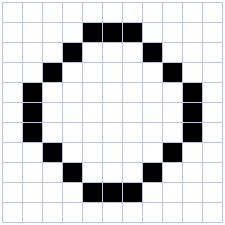
\includegraphics[height=2.5cm]{img/bitmap.jpg}
	}
	\subfloat[Vectorial]{
	          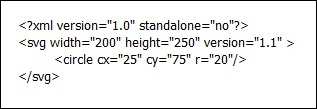
\includegraphics[height=2.5cm]{img/vectorial.jpg}
	}
	\caption{Representación de un circulo}
\end{figure}

Existe formatos tan comunes como pdf que son híbridos, es decir, algunas regiones del documento son representadas de forma vectorial y otras como mapas de bit.
\newpage

Si nos centramos en el proceso de rasterización, los formatos en mapa de bits son mucho más ligeros que los vectoriales, esto se debe a que existe una relación casi directa entre las celdas del mapa de bit y los píxeles de pantalla. 
\newline 

Sin embargo, como la resolución de una mapa de bit esta implícito en el formato, en algunos casos pueden provocarse errores en la rasterización conocidos como aliasing. Estos errores se producen cuando se adapta a la resolución de la pantalla donde se va a visualizar. Para corregir esta problemática, existen distintos tipos de filtros conocidos como \textbf{antialiasing}, los cuales son capaces de detectar aquellos píxeles conflictivos  y cambiar su color a uno más apropiado. 

	\begin{figure}[h]
	\centering	
	\subfloat[Aliasing I]{
	          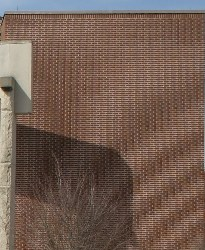
\includegraphics[width=4cm]{img/AliasedBrick0.jpg}
	}
	\subfloat[Anti-Aliasing]{
	          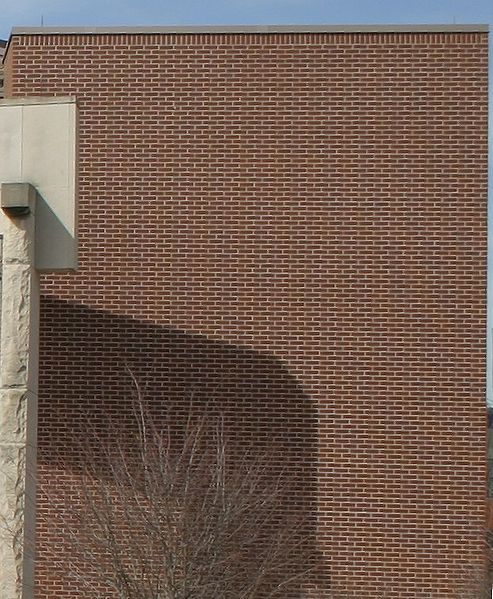
\includegraphics[width=4cm]{img/AliasedBricks1.jpg}
	}
	\caption{Efectos del aliasing y antialiasing sobre una pared de ladrillos}
	\end{figure}


La computación gráfica también abarca las animaciones o secuencias de imágenes. Como hemos visto, existe una relación directa entre un formato bidimensional y una imagen, por este motivo, para crear animaciones necesitaremos tener secuencias de formatos bidimensionales.
\newpage

	\begin{figure}[!h]
	\centering	
          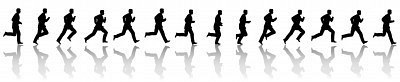
\includegraphics[height=1.5cm]{img/animacion.jpg}
	\caption{Animación de una persona corriendo}
	\end{figure}


Los videojuegos intentan crear animaciones cercanas a la realidad, proyectando los elementos en la pantalla de la forma más realista posible. Lo que implica tener en cuenta desde dónde se proyecta la imagen que estamos capturando y la iluminación existente. La única forma de poder recrear esta situación con formatos en 2D sería tener un numero infinito de imágenes, por este motivo se usan los formatos en 3D.

	\begin{figure}[h]
	\centering	
	\subfloat[Pacman (1980)]{
	          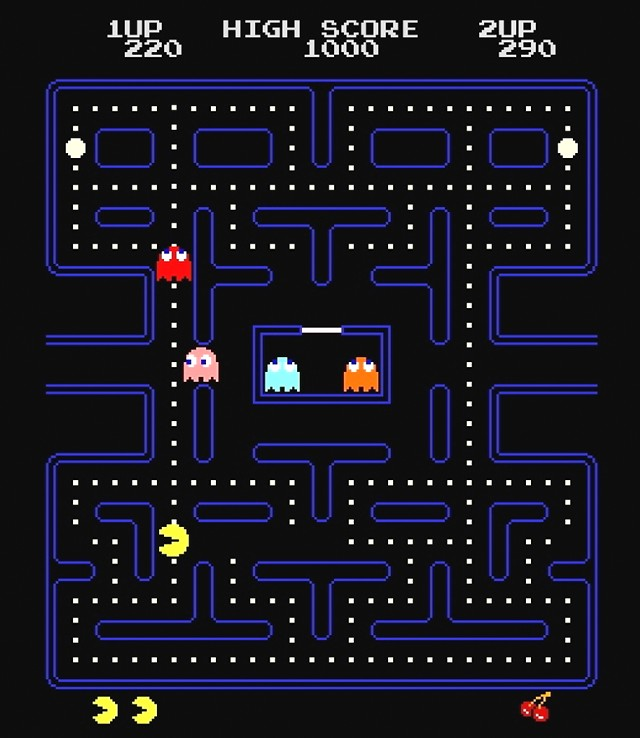
\includegraphics[height=5cm]{img/pac-man.jpg}
	}
	\subfloat[Super Mario Bros (1985)]{
	          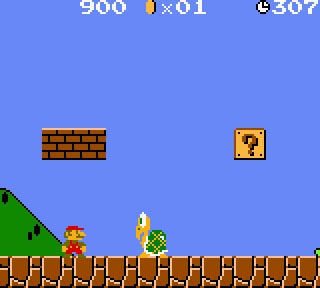
\includegraphics[height=5cm]{img/super-mario-bros.jpg}
	}

	\subfloat[Prince of persia (1989)]{
	          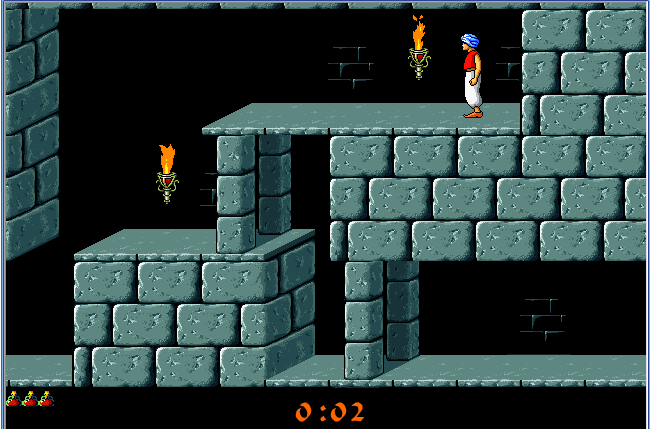
\includegraphics[width=7cm]{img/prince_of_persia.png}
	}
	\caption{Evolución de videojuegos con formato 2D}
	\end{figure}


\section{Formatos tridimensionales (3D)}

Los complejidad de los formatos 3D es muy superior comparada con los formatos 2D. Para representar una escena se ha de indicar cada uno de los elementos existentes, la iluminación y qué parte de esa escena va a ser proyectada en la pantalla. Al pensar en una escena cualquiera, por ejemplo una casa, los elementos que lo componen serían las distintas habitaciones, armarios\ldots\ La iluminación variará en función de las luces que estén encendidas y la luz que entre por las ventanas. La proyección de la escena sobre la pantalla no sólo dependerá de los elementos y la iluminación, también será influida por la posición en el que se sitúe el espectador. No vemos lo mismo si estamos sentados en el sillón o tumbados en la cama.

\subsection{Mallas}

Cada elemento de una escena es representado mediante polígonos. El conjunto de los polígonos que componen un elemento se conoce como malla o en ingles, \texttt{mesh}. En computación gráfica estos polígonos se reducen a cuadriláteros o triángulos\footnote{Actualmente los dispositivos móviles tan sólo tratan con mallas definidas por triángulos}. Cada polígono, conocido por cara o face, está formado a su vez  por tres o cuatro vértices para formar un triángulo o un cuadrado respectivamente.

\begin{figure}[h]
	\centering
	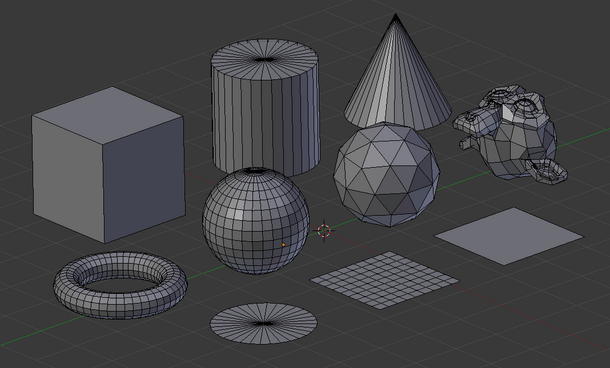
\includegraphics[width=12cm]{img/mallas.png}
	\caption{Ejemplos básicos de mallas}
\end{figure}

Ahora ya sabemos que el contorno de cada una de los elementos de la escena se realiza mediante mallas, pero desconocemos el color de la misma. Para dar color a cada una de las caras de una malla, se ha de indicar el color de cada uno de los vértices que lo componen. 


Indicar el color de los distintos vértices no es suficiente, también se han de indicar otras propiedades como son el sombreado y si aplican o no texturas, conceptos, que explicamos a continuación.

\begin{description} 

\item [Sombreado:] es un algoritmo mediante el cual se indica cómo se va a calcular el color de los píxeles intermedios dentro de cada polígono. Los principales algoritmos son:

\begin{itemize}
\item \textbf{Flat:} todos los píxeles del polígono tendrán un único color, por lo que todos los vértices también han de tener ese mismo color. Debido a su simplicidad su coste computacional es muy bajo pero los resultados son muy pixelados y por tanto de peor calidad gráfica.
\item \textbf{Gouraud:} de mayor detalle que el anterior, se centra en los vértices de cada polígono, calculando el color de cada punto de la superficie interpolando los colores de cada vértice.
\item \textbf{Phong:} es el  algoritmo más preciso para calcular el color por cada píxel, en el cual se interpolan los vectores normales de sus vértices. Por contra su coste es bastante más elevado que Gouraud. Cuando los polígonos de los elementos de la escena son más pequeños que un píxel, los algoritmos Gouraud y Phong tienen el mismo resultado.
\end{itemize}

\begin{figure}[h]
	\centering
	\subfloat[Flat]{
	          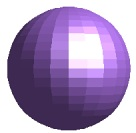
\includegraphics[height=3.3cm]{img/flat.jpg}
	}	
	\subfloat[Gouraud]{
	          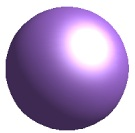
\includegraphics[height=3.3cm]{img/gourad.jpg}
	}
	\subfloat[Phong]{
	          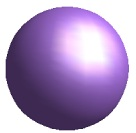
\includegraphics[height=3.3cm]{img/pong2.jpg}
	}
	\caption{Esfera con los tres tipos de sombreado}
\end{figure}


\item [Texturas:] son imágenes que se aplican sobre la malla dándole un mayor realismo. Al aplicar una textura se ha de indicar su mapeo, es decir, cómo se traslada la imagen sobre la malla. Para ello se usan las siguientes propiedades:

\begin{itemize}
\item \textbf{Repeating:} indica si la imagen se ha de repetir sobre los ejes.
\item \textbf{Clamping:} indica si se ha de extender el último píxel de la imagen sobre los ejes.

\begin{figure}[h!]
\centering	  
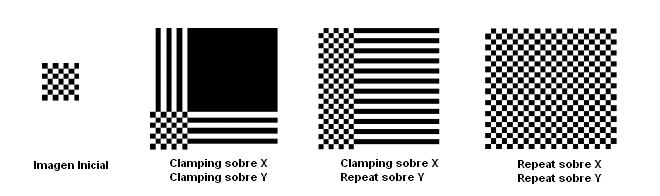
\includegraphics[width=12cm]{img/ClampingRepeatMapping.jpg}
\caption{Efectos de clamping y repeating}
\end{figure}

\item \textbf{UV Mapping:} indica la correspondencia entre los vértices de la malla y los píxeles de la imagen. En función de si la malla es un plano, cubo, tubo o esfera se conocen como flat, cube, tube o sphere mapping.
\begin{figure}[h]
	\centering	  
	\subfloat[Cube mapping]{
	          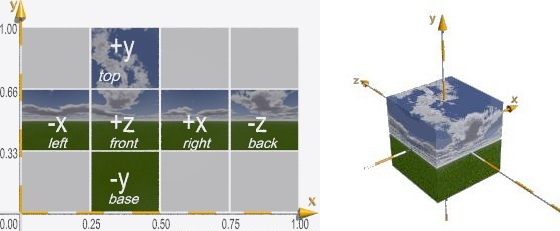
\includegraphics[height=2.8cm]{img/CubeMapping.jpg}
	}
	\subfloat[UV mapping]{
	          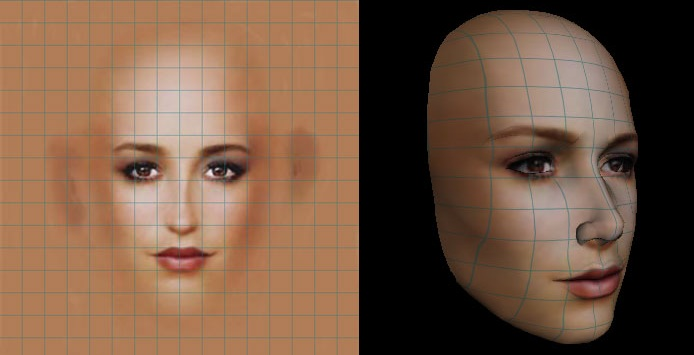
\includegraphics[height=2.8cm]{img/textura_uvMapping.jpg}
	}
	\caption{Ejemplos de mapeos}
\end{figure}
\label{funcionesMapeo}
\item \textbf{Función de mapeo:} determina cómo afecta la textura sobre el objeto. Entre las funciones más conocidas podemos destacar:


\begin{itemize}
\item \textbf{Dispacement mapping:} técnica utilizada para deformar una malla mediante una textura. Consiste en desplazar cada vértice de la malla una distancia determinada por la imagen asociada a la textura. 

\begin{figure}[h]
\centering	  
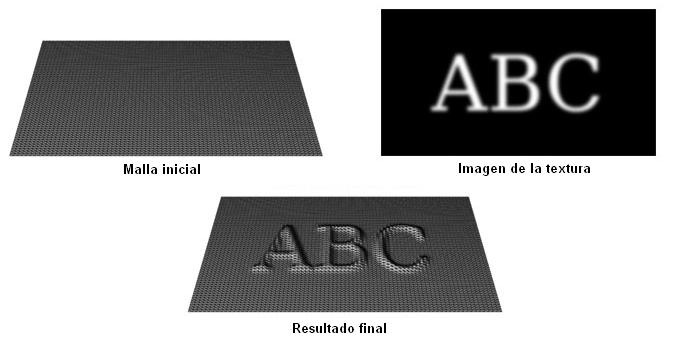
\includegraphics[height=4.5cm]{img/Displacement.jpg}
\caption{Ejemplo de displacement mapping}
\end{figure}

\item \textbf{Normal mapping:} técnica que consiste en modificar las normales\footnote{Las normales o vector normal es el vector perpendicular al plano formado por los vértices.} de una malla, aplicando un desplazamiento definido por una textura, de esta forma se consigue un mayor detalle con menos vértices. Hay que tener en cuenta que al no modificar la geometría del objeto tampoco lo harán sus sombras.\begin{figure}[ht]
\centering	  
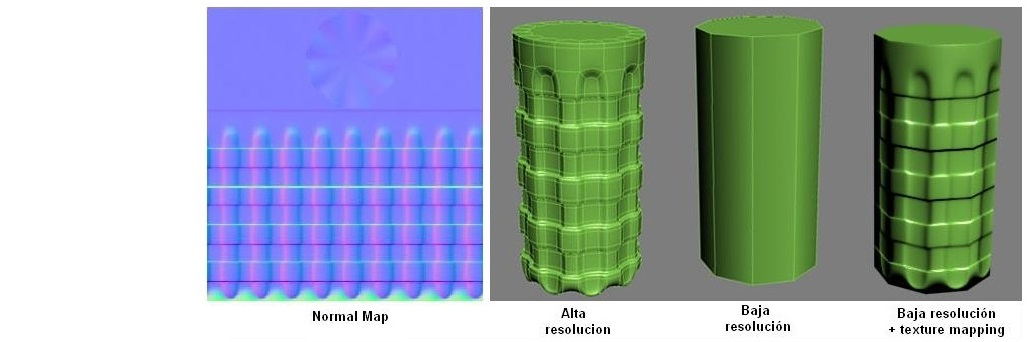
\includegraphics[height=4cm]{img/NormalMapping.jpg}
\caption{Ejemplo de normal mapping}
\end{figure}
 

\end{itemize}
\end{itemize}

\end{description}

Otras de las ventajas que nos ofrece los modelos 3D es la posibilidad de articular las mallas mediante un nuevo concepto, la armadura. 
\newline

\label{sec:armadura}
La armadura es una especie de esqueleto, compuesto por varias articulaciones, que al moverse, se traslada dicho movimiento sobre los vértices cercanos que la componen. En las películas de animación estas armaduras son creadas a partir de unos trajes que contienen multitud de sensores, los cuales transmiten información sobre cualquier movimiento que realizan.
\begin{figure}[h]
	\centering	  
	\subfloat[Armadura]{
	          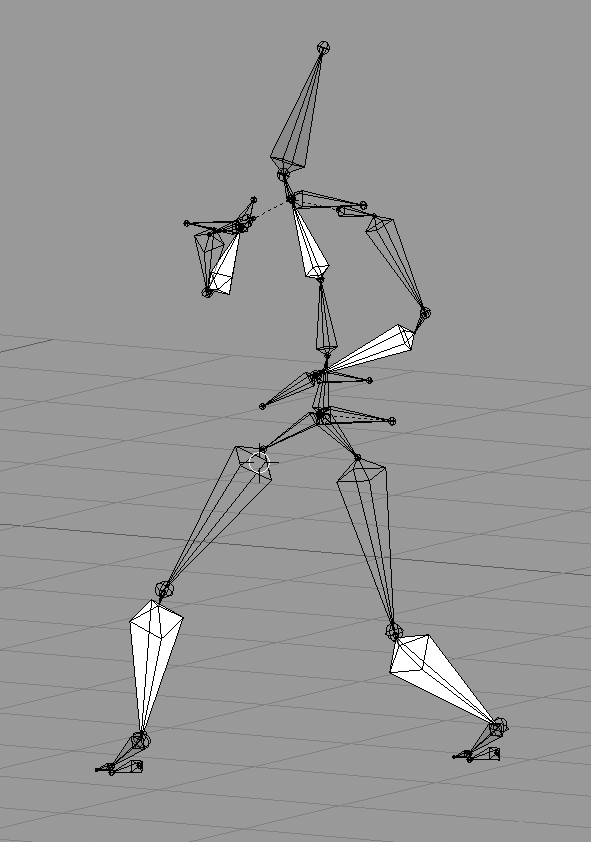
\includegraphics[height=5cm]{img/armadura1.png}
	}
	\subfloat[Pose 1]{
	          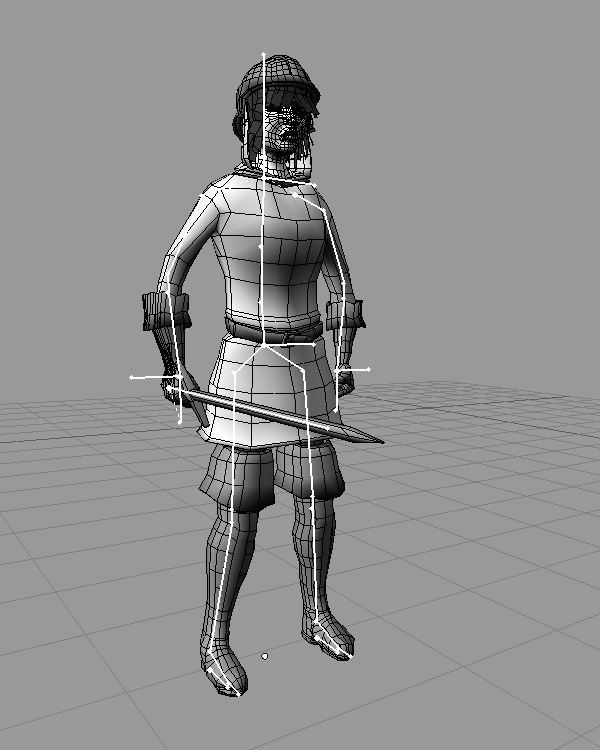
\includegraphics[height=5cm]{img/armadura2.png}
	}
	\subfloat[Pose 2]{
	          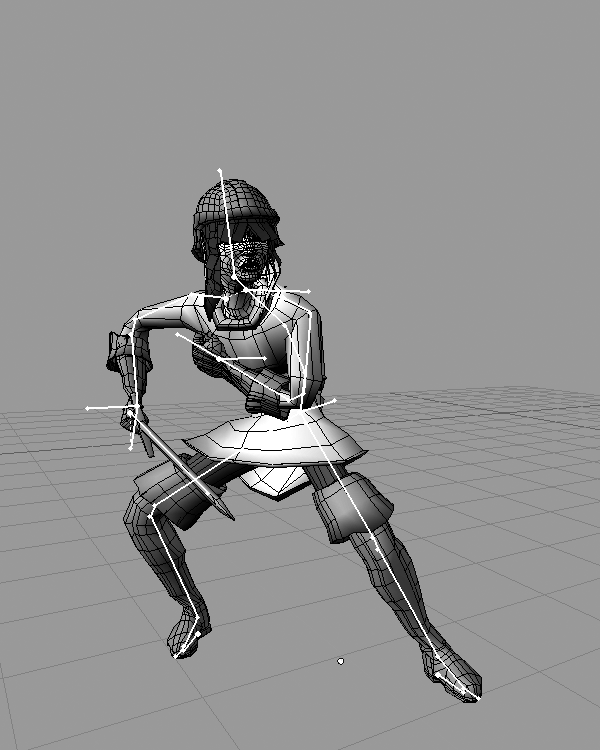
\includegraphics[height=5cm]{img/armadura3.png}
	}
	\caption{Armadura sobre un guerrero}
\end{figure}




\subsection{Cámaras}

Mediante el concepto de cámara se indica el lugar desde el cual, la escena va a ser proyectada sobre la pantalla. De cada una de las cámaras de una escena hemos de conocer su posición y orientación mediante los siguientes parámetros:
\begin{itemize}
	\item  \textbf{Eye:} define la posición de la cámara en el espacio.
         \item  \textbf{Center:} define el punto al cual estamos mirando.
         \item  \textbf{Up:} define el vector vertical a la cámara.
	\begin{figure}[!h]
		\centering
	         	 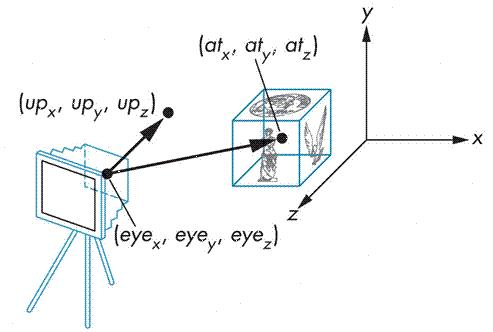
\includegraphics[width=7.5cm]{img/glulookat.jpg}
		\caption{Posición y orientación de una cámara}
	\end{figure}
\end{itemize}

También hemos de establecer los siguientes parámetros de la cámara, a través de los cuales se determinará el área visible de la escena. 
\begin{itemize}
\item  \textbf{Fovt:} define el ángulo de apertura de la cámara 
\item  \textbf{Aspect:} define la proporción entre ancho y alto de la imagen (16:9, panorámico, 4:3, etc)
\item \textbf{ Near:} define la distancia al plano de corte cercano a la cámara
\item  \textbf{Far:} define la distancia al plano de corte más alejado de la cámara.
\end{itemize}
\begin{figure}[!h]
	\centering
	          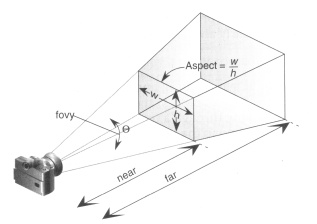
\includegraphics[width=7cm]{img/gluperspective.png}
	\caption{Frustrum de una cámara}
\end{figure}

\subsection{Luces}

En cada escena hay que indicar los distintos focos de luz existentes, por cada uno de ellos se han de especificar las siguientes propiedades:

\begin{itemize}
	\item \textbf{Color:}  de la luz que emite el foco.
	\item \textbf{Intensidad:} con la que la luz es emitida y cómo se va atenuando con la distancia.
	\item \textbf{Tipo de luz:}
	\begin{itemize}
		\item Directional light: es un tipo de luz ubicada en el infinito, por ejemplo el Sol.
		\item Point light: es un tipo de luz posicionada en un punto que emite luz en todas las direcciones, por ejemplo, una bombilla.
		\item Spot light: es un tipo de luz similar al Point Light pero sólo emite protones bajo una superficie conoidal, determinada por un vector direccional y el angulo de corte. Un ejemplo claro de este tipo de luz es un linterna.
	\end{itemize}
	
	\begin{figure}[!h]
	\centering
	\subfloat[Tipos de luces]{
	          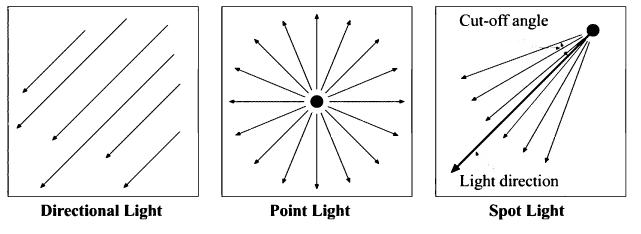
\includegraphics[width=7cm]{img/typeoflight.jpg}
	}

	\subfloat[Iluminación aplicada a un plano]{
	          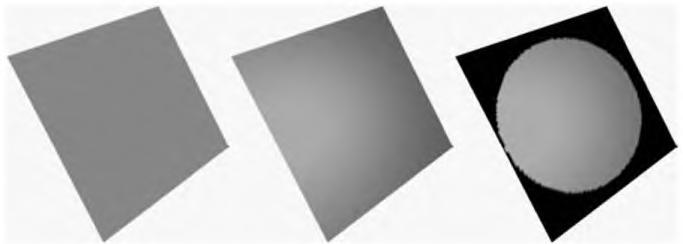
\includegraphics[width=7cm]{img/typeoflight2.jpg}
	}
	\caption{Tipos de luces y el efecto sobre un plano}
	\end{figure}
\end{itemize}


\section{Modelos de iluminación}\label{modeloIluminacion}

En puntos anteriores se han determinado distintos elementos que forman una escena, hemos identificado el color de las mallas, pero el color real en la escena depende de muchos factores. Si observamos un objeto de color blanco a plena luz del día, lo veremos blanco, pero si ese mismo objeto lo encontramos en una habitación con una luz roja, diremos que es rojo, por lo tanto, el color de los focos de luz existentes es un factor a tener en cuenta en la iluminación de una escena. También hay que tener en cuenta que la luz emitida por los focos puede estar siendo bloqueada por otras mallas de la escena, provocando sombras. Los modelos de iluminación son los responsables de determinar el color real del objeto en función de estos factores y muchos otros.
\newline

Para poder entender los modelos de iluminación se exponen a continuación una serie de conceptos de óptica básicos y cómo son trasladados a una computadora.

\subsection{Conceptos ópticos básicos}

La óptica puede ser estudiada pensando en su geométrica, física o cuántica, nos centraremos en la geométrica que es la utilizada en las computadoras para simular el comportamiento de la luz.
\newline

\begin{figure}[h]
	\centering
	          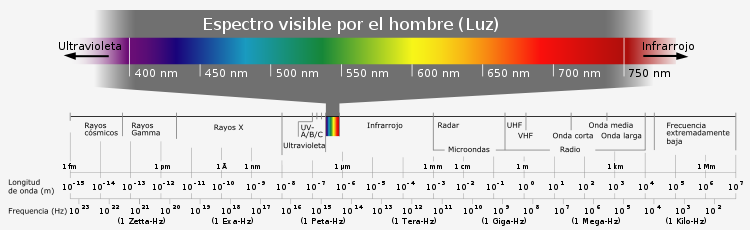
\includegraphics[width=14cm]{img/espectroElectromagnetico.png}
	\caption{Espectro electromagnético de la luz}
\end{figure}

La óptica geométrica está fundamentada en la teoría de los rayos de luz. Esta teoría considera que todo objeto visible emite rayos rectos de luz en todas direcciones a su alrededor. Cuando estos rayos inciden sobre otros cuerpos, se presentan los siguientes fenómenos ópticos:

\begin{description}
\item [Reflexión:] el rayo de luz es proyectado en sentido contrario al que incide sobre el objeto. Dependiendo del material del objeto existen dos tipos de reflexión:
\begin{itemize}
	\item \textbf{Difusa:} el rayo incidente es reflejado en un amplio abanico de direcciones con intensidades equivalentes, debido a rugosidades en el material. 
	\item \textbf{Especular:} el rayo incidente es reflejado en una única dirección y con el mismo ángulo con el que incide en el objeto.  
\end{itemize}

La reflexión lleva asociada una pérdida de intensidad lumínica en función de las características del objeto con el que haya colisionado el rayo de luz.  Cuanta más luz retenga el objeto, menor será la intensidad del rayo reflejado.

\begin{figure}[h]
	\centering
	\subfloat[Difusión]{
	          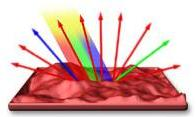
\includegraphics[width=5cm]{img/reflexion_difusa.jpg}
	}
	\subfloat[Especular]{
	          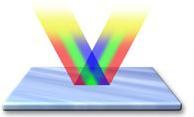
\includegraphics[width=5cm]{img/reflexion_especular.jpg}
	}
	\caption{Fenómenos de reflexiones difusa y especular}
\end{figure}
\item [Refracción:] es el cambio de dirección que experimenta un rayo de luz al pasar de un medio a otro. Este cambio de dirección es lo que provoca que veamos torcido un lápiz al ser sumergido en el agua.
\begin{figure}[h]
	\centering
	          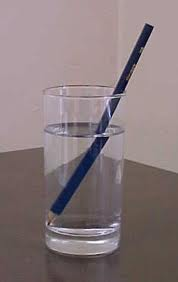
\includegraphics[width=4cm]{img/refraction.jpg}
	\caption{Fenómeno refracción sobre el agua}
\end{figure}
\item [Absorción:] cuando un rayo luminoso se propaga, va disminuyendo paulatinamente su intensidad, siendo absorbida poco a poco por el entorno, dotándole de color.  Si un objeto absorbe todos los colores de la luz menos el verde, el ojo humano percibirá dicho objeto de color verde.
\end{description}


\subsection{Aproximación a un modelo computacional}

Hasta el momento hemos hablado del color de las luces y las mallas, lo cual es una simplificación. En un modelo computacional hemos de hablar de la cantidad de luz que absorben las mallas o emiten las luces. El espectro luminoso de la luz se representa por el modelo RGB, es decir, los niveles de rojo, verde y azul. 
\begin{figure}[h!]
	\centering	  
	\subfloat[Cubo de luz]{
	          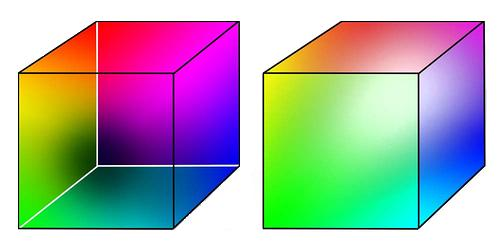
\includegraphics[height=4cm]{img/RGBCube.jpg}
	}
	\subfloat[Colores principales]{
	          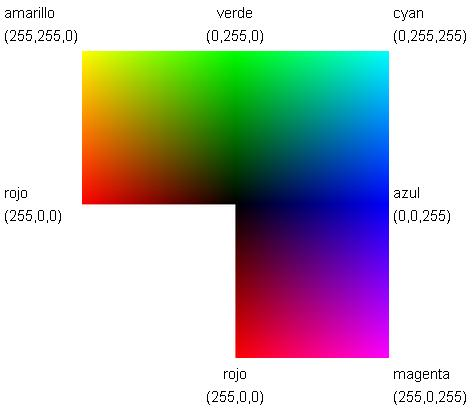
\includegraphics[height=4cm]{img/RGBCube2.jpg}
	}
	\caption{Visualización del espectro de luz sobre un cubo RGB}
\end{figure}

La luz es descompuesta en los siguientes tipos de luces:
\begin{itemize}
\item \textbf{Luz ambiental:} es aquella que proviene de una fuente que ha sido tan disipada por el entorno que es imposible determinar su dirección.
\item \textbf{Luz de difusión:} es aquella sobre la que será aplicado el fenómeno de difusión generando objetos con un contorno suavizado y pudiendo observar su forma tridimensional.
\item \textbf{Luz especular:} es aquella sobre la que será aplicado el fenómeno de reflexión especular, generando brillos en los objetos.
\item \textbf{Luz de emisión:} se corresponde con la luz que emite un objeto. Por motivos de simplificación, suele tratarse como un incremento de la luz ambiental específica para dicho objeto.
\end{itemize}

Aplicando este modelo a una luz en nuestro escenario, hemos de establecer el nivel de luz ambiental, de difusión y especular sobre cada uno de los focos de luz y sobre cada objeto. Además deberemos saber cúal será su comportamiento ante el fenómeno de absorción de la luz, es decir, cuáles son los niveles de luz ambiental, difusión y especular que absorberá, además de la luz de que emite el objeto por si mismo. 

\subsection{Clasificación de modelos de iluminación}

Ahora que conocemos las propiedades ópticas básicas, podemos centrarnos en el concepto de modelo de iluminación, a través del cual, se va a determinar cómo se va a simular en la computadora el comportamiento de la luz sobre los objetos. 
\newline 

Los modelos se clasifican principalmente por el tipo de iluminación. En el modelo de \textbf{iluminación directa} únicamente están implicados los rayos de luz procedentes de una fuente de luz y que colisionan con un objeto. Ahora sabemos que este rayo de luz puede sufrir el fenómeno de reflexión, modificando las propiedades del rayo, el cual puede volver a colisionar con otros objetos. Los rayos procedentes de la reflexión son descartados en modelos de iluminación directa, pero en los que se fundamentan los modelos de \textbf{iluminación global}.
\newline

Los métodos de iluminación global generan escenas difícilmente distinguible de la realidad, es lo que se conoce como foto-realismo pero no son aplicables al mundo de los videojuegos debido a su elevado coste computacional. Están surgiendo nuevos modelos de iluminación híbridos, dando origen al término de  foto-realismo animado. 

\begin{figure}[h]
	\centering
	          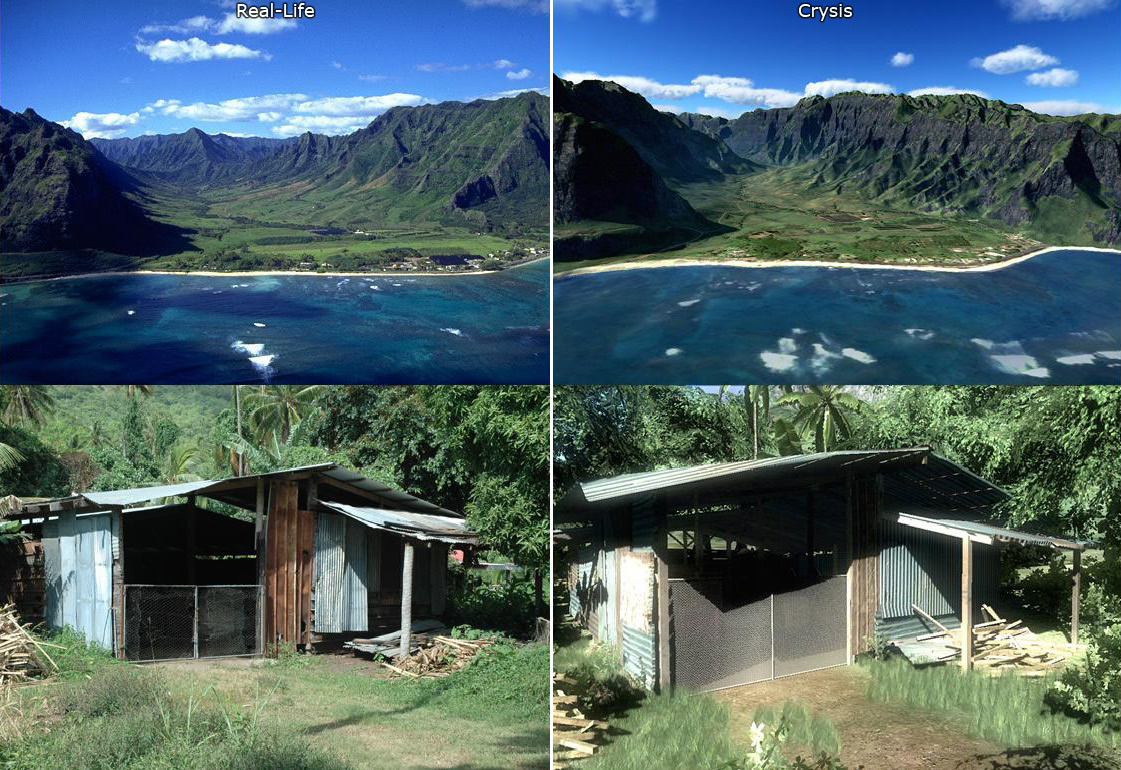
\includegraphics[width=11cm]{img/fotorealismo.jpg}
	\caption{Imágenes del juego Crysis 2 comparadas con la realidad}
\end{figure}

A continuación se muestra un listado de modelos de iluminación más populares, entre los cuales nos centraremos en Phong y Radiosity:

\begin{itemize}
\item \textbf{Lambert:} modelo de iluminación directa, ideal para superficies plásticas ya que esta basado en superficies difusas perfectas, por lo tanto, sobre el modelo de reflexión especular.
\item \textbf{Oren-Nayar:} modelo de iluminación directa, ideal para superficies fibrosa como ropa, madera y pelo. Está basado en superficies difusas borrosas, es decir, un modelo de reflexión de difusión.
\item \textbf{Phong:} modelo de iluminación directa basado en superficies especulares, ideal para elementos con superficies parecidas a un espejo sin llegar a serlo, como pinturas con brillo y metales.
\item \textbf{Radiosity:} modelo de iluminación global basado en el nivel de calor absorbido por los elementos puramente difusos.
\item \textbf{Ray-tracing:} modelo de iluminación global que simula el trazado de rayos de luz desde el observador. Por cada uno de los rayos simulados se tiene en cuenta los fenómenos de reflexión y refracción.
\end{itemize}

\subsection{Modelo de iluminación de Phong}

Es un modelo de iluminación directa, desarrollado en 1973 por Bui Tuong Phong en la universidad de Utah, basándose en la combinación de reflexión especular y difusión, nivel de brillo de la superficies, iluminación ambiental y atenuación de la luz. 
\newline 

En el modelo de iluminación de Phong, el color en un punto $P$ en una superficie cuyo material está definido por $K$, donde 
      $$ K = \{ K_{ambiental}, K_{difusión}, K_{especular} \}$$ 
Y sobre el que se aplica una luz con una intensidad definida por $ L $ donde 
$$ L = \{ L_{ambiental}, L_{difusión}, L_{especular}\} $$ 
Se determina por la suma de las intensidades de luz reflejadas, es decir: 
$$ Color = Color_{ambiental} + Color_{diffusión} + Color_{especular} $$ 

\begin{figure}[h]
	\centering
	          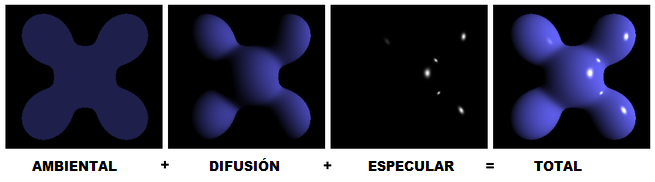
\includegraphics[width=11cm]{img/PhongComponent.png}
	\caption{Modelo de iluminación de Phong}
\end{figure}


Para el calculo del color final del objeto se tendrán en cuenta los vectores formados por la posición de la luz, el observador y el punto de colisión entre el rayo de luz y el objeto, a este punto lo llamaremos $P$. A partir de estos tres puntos se han de calcular:
\begin{itemize}
\item El vector normal de la superficie en $ P $ se define como $  \vec{n} $.
\item El vector entre el punto donde se ubica la cámara y el punto $P$ se define como   $ \vec{v}$.
\item El vector entre el origen de la luz y el punto $ P $ se define como  $  \vec{l} $ y forma un angulo $\theta$ con respecto a la normal.
\item El vector de la luz reflejado en el mismo angulo $\theta$ respecto a la normal se define como $ \vec{r}$.
\end{itemize}

\begin{figure}[h!]
	\centering
	          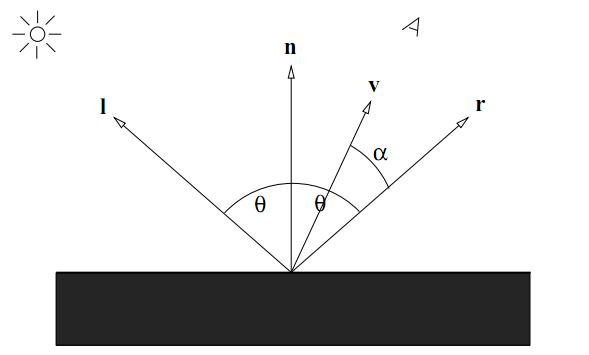
\includegraphics[width=7cm]{img/phongVector.jpg}
	\caption{Vectores utilizados en el modelo Phong}
\end{figure}

\begin{description}
\item [El componente ambiental] se corresponde con el producto de la intensidad de la luz ambiental sobre los materiales de emisión y ambiental, es decir: 
	$$ Color_{ambiental} = ( K_{ambiental} + K_{emision} ) * L_{ambiental} $$

\item [El componente de difusión] se calcula con la intensidad de la luz de difusión, aplicada al material correspondiente, pero teniendo en cuenta el ángulo existente entre la normal y el vector de la luz. Cuanto más pequeño sea el ángulo entre los vectores, mayor será su producto escalar, por lo que recibirá más luz. Si el punto de luz está muy alejado, el producto vectorial puede resultar negativo, por lo que no llegará luz y el valor se redondeará a cero. 
	$$ Color_{difusión} = K_{difusión} * L_{difusión} *max(\vec{n} \cdot \vec{l}, 0)$$

\item [El componente especular] depende del punto de vista del observador sobre el rayo reflejado. El producto escalar entre ambos vectores es tratado de igual forma que en el componente de difusión.
	$$ Color_{especular} = K_{especular} * L_{especular} *max( \vec{r} \cdot \vec{v}, 0)$$

\end{description}

\subsection{Modelo de iluminación por radiosidad}

La radiosidad se fundamenta en el estudio térmico de la luz debido a la vibración de los fotones, determinando que una superficie estará más iluminada cuanto más fotones choquen contra ella o lo que es lo mismo, tenga un mayor nivel de radiosidad. 
\newline 

Nos encontramos con un modelo de iluminación global y con un comportamiento de los objetos puramente difuso. Todos los rayos de luz son reflejados de forma homogénea y con la misma intensidad en todas direcciones, restándole parte de su calor o intensidad limúnica inicial, debido al fenómeno de absorción.
\newline 

\begin{figure}[h!]
	\centering
	          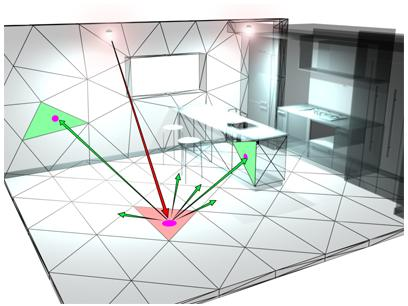
\includegraphics[width=7cm]{img/radiositymodel.jpg}
	\caption{Modelo de radiosidad donde podemos observar en rojo una luz directa que es reflejada y sus rayos indirectos que se muestran en verde}
\end{figure}

La radiosidad en un determinado punto, $ B_i $ se define cómo la energía por unidad de área que emite una superficie por unidad de tiempo, que no es más que la suma de la luz emitida por la superficie y la energía reflejada proveniente de otras superficies:
	$$ B_I = E_i + R_i \sum B_jF_{ij} $$ 
Donde:
\begin{itemize}
\item $E_i$: energía emitida por la superficie $i$.
\item $R_i$: capacidad de reflexión de la superficie $i$.
\item $B_j$: energía transmitida de la superficie $j$ sobre $i$.
\item $F_{ji}$: factor de forma entre $i$ y $j$ que mide la cantidad de energía que emitida por $j$ llega a $i$.
\end{itemize}

Finalmente, en cada punto de la escena, se calcularán los componentes ambiental, especular y de difusión del escenario, basándose en la intensidad de luz, calculada previamente en el modelo de radiosidad.
\newline

\begin{figure}[h!]
	\centering
	          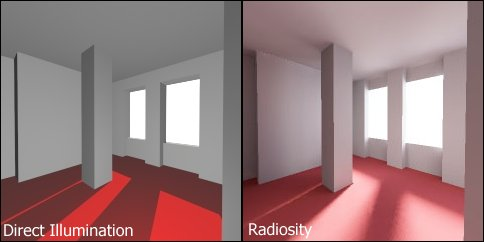
\includegraphics[width=10cm]{img/radiosity_comparison.jpg}
	\caption{Comparativa de una escena procesada con radiosidad y phong}
\end{figure}

Las ventajas y desventajas de este modelo de iluminación son las siguientes:
\begin{itemize}
\item La calidad de la imagen es cercana a la realidad.
\item El tiempo de procesamiento es elevado.
\item Se puede generar un procesamiento progresivo, es decir, en cada paso se puede ver la escena, incrementando su realismo cuantos más pasos se realicen. Cada paso  consiste en calcular los nuevos rayos generados por la reflexión.
\item La radiosidad de la escena no cambia ante cambios de cámara por lo que no ha de ser recalculada por los movimientos de la cámara.
\item La radiosidad de la escena cambia al cambiar la posición de cualquier elemento de la escena, pudiendo cambiar la trayectoria de algunas rayos y por lo tanto, la radiosaidad de las superficies. Este es el motivo por el cual no resulta útil en el desarrollo de videojuegos.
\item Para calcular la radiosidad de la escena no se usan los polígonos que componen las distintas mallas debido a su elevado número, para acelerar este cálculo se utilizan unas superficies más amplias. Debido a esta simplificación se pueden ocasionar algunos errores en el calculo de la radiosidad.
\end{itemize}

\section{Librerías de computación gráfica}

Debido a la complejidad de las escenas en tres dimensiones, surgen unas librerías de uso común para simplificar estas tareas al desarrollar aplicaciones. Las librerías más conocidas en el mercado son:
\begin{itemize}
\item La desarrolla por Microsoft, \textbf{DirectX}, que está limitada para entornos con un sistema operativo Windows.
\item Las basadas en el API de \textbf{OpenGL}, implementadas para sistemas operativos Unix, Linux, Windows, etc.
\end{itemize}
\begin{figure}[h!]
	\centering	  
	\subfloat[DirectX]{
	          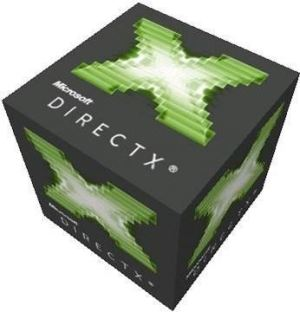
\includegraphics[height=2.5cm]{img/DirectX-Logo.jpg}
	}
	 \hspace*{1cm}
	\subfloat[OpenGL]{
	          
\includegraphics[height=2.5cm]{img/OpenGL_logo.png}
	}
	\caption{Logotipos de las librerías}
\end{figure}

DirectX no está soportada en Android, por lo que nos centraremos en OpenGL, para ser más exactos, sobre \textbf{OpenGL ES}, una versión más optimizada para los sistemas con un bajo nivel de procesamiento. En esta versión se han simplificado sus operaciones pero sin alterar su funcionalidad. Existen tres versiones:
\begin{description}
\item [OpenGL ES 1.0:] procede de OpenGL 1.3 e implementa un modelo de iluminación de Phong en el pipeline fijo del microprocesador de la tarjeta gráfica.
\item [OpenGL ES 1.1:] es una evolución de la 1.0 añadiendo ciertas mejoras de OpenGL 1.5. 
\item [OpenGL ES 2.0:] procede de OpenGL 2.0, que da un gran salto al incluir un pipeline dinámico, al que poder incorporar en algunos de sus pasos los shaders, a partir de los cuales se puede crear un modelo de iluminación acorde a las necesidades de cada proyecto.
\end{description}

 Los shaders son códigos fuente compilados e interpretados por los microprocesadores de las tarjetas gráficas en tiempo de ejecución. Están escritos en un nuevo lenguaje llamado GLSL (Graphics Library Shaders Languaje). Para entender cómo funcionan hemos de conocer la estructura de OpenGL 2.0.

\subsection{OpenGL 2.0}

Toda tarjeta gráfica que soporte OpenGL 2.0 estará compuesta por un pipeline con una estructura similar al mostrado en el siguiente gráfico. Se han identificado con cajas sombreadas aquellas fases en las que es posible insertar shaders.
\newline

\begin{figure}[h!]
\centering
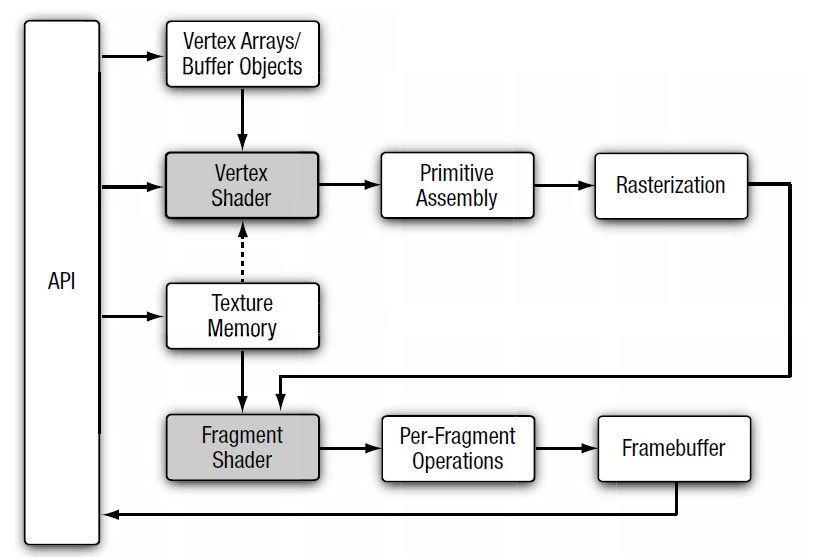
\includegraphics[width=11.5cm]{img/OpenGL_Pipeline2.jpg}
\caption{Pipeline en OpenGL ES 2.0}
\end{figure}

La primera fase \texttt{Vertex Array/Buffer Object} se corresponde a la adaptación de los datos definidos en el API a la estructura hardware dependiente de la tarjeta, por este motivo no haremos hincapié en ella.

\subsubsection{Vertex Shader}

En esta segunda fase se realizan operaciones sobre los vértices de cada malla, de uno en uno, por lo que se desconoce la forma de la malla. Las operaciones más frecuentes son transformaciones afines, proyecciones, transformaciones de color, coordenadas de textura e iluminación. La entrada de esta fase está constituida por:
\begin{itemize}
\item \textbf{Atributos:} propiedades inherentes a los vértices (coordenadas de textura, vector normal\ldots) que pueden ser definidas o creadas por la aplicación de OpenGL para cada vértice. 
\item \textbf{Uniforms:} propiedades generales a todos los vértices que pueden ser definidas por la aplicación de OpenGL como una constante.
\item \textbf{Samplers:} se corresponden con las texturas, siendo opcionales en esta fase.
\end{itemize}

Es obligatorio definir el \textbf{GL\_Position}, que se corresponde con la posición final del vértice. Las variables GL\_PointSize y GL\_FrontFacing son opcionales. Indican el tamaño en píxeles del vértice y la ecuación del plano de corte respectivamente. Para comunicarse con otras fases del pipeline se utilizan variables de tipo varying.
\newline

A modo de ejemplo, a partir de un vertex shaders, podríamos ser capaces de modificar los vértices de una malla junto con una textura, aplicando la técnica de dispacement mapping, descrita en la página 39, cuando se definía el concepto de malla.

\begin{figure}[H]
\centering
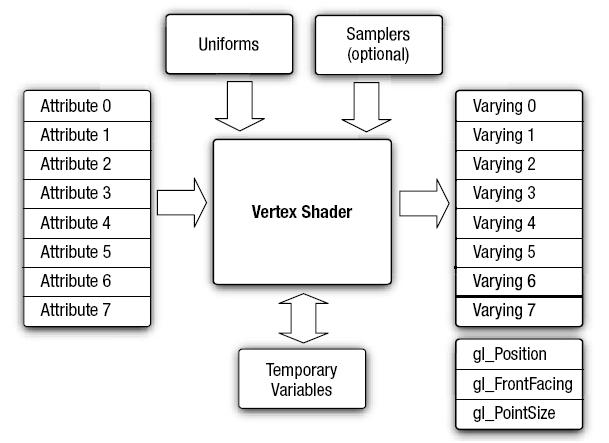
\includegraphics[width=11cm]{img/VertexShader.jpg}
\caption{OpenGL ES 2.0 Vertex Shaders}
\end{figure}

\subsubsection{Primitive Asemmbly y rasterización}

La tercera fase consisten en agrupar los vértices formando puntos, lineas o polígonos para después ejecutar la rasterización y obtener los fragmentos que van a componer la imagen. 

\begin{figure}[!h]
\centering
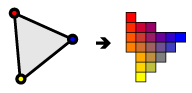
\includegraphics[width=4.5cm]{img/rasterization.png}
\caption{Ejemplo de rasterización}
\end{figure}

\subsubsection{Fragment Shader}

En la cuarta fase, programable mediante un shader, recibe los fragmentos obtenidos en la fase anterior. Sobre estos segmentos se pueden aplicar operaciones de mapeo de texturas, mezcla de colores, efecto de niebla\ldots
\newline

El objetivo del fragment shaders es conseguir el color del fragmento, almacenado en la variable \textbf{GL\_FragColor}, utilizando un modelo de iluminación con los siguientes datos y las variables de tipo uniform y varying, definidas previamente:
\begin{itemize}
\item \textbf{GL\_FragCoord:} indica las coordenadas del fragmento.
\item \textbf{GL\_FontFacing:} indica si el fragmento está oculto por otro fragmento.
\item \textbf{ GL\_PointCoord:} coordenadas de dispersión aplicado sobre las partículas\footnote{El concepto de partículas esta fuera del alcance del proyecto y es usado para simular objetos muy dinámicos como son fuegos artificiales.}.
\end{itemize}

\begin{figure}[H]
\centering
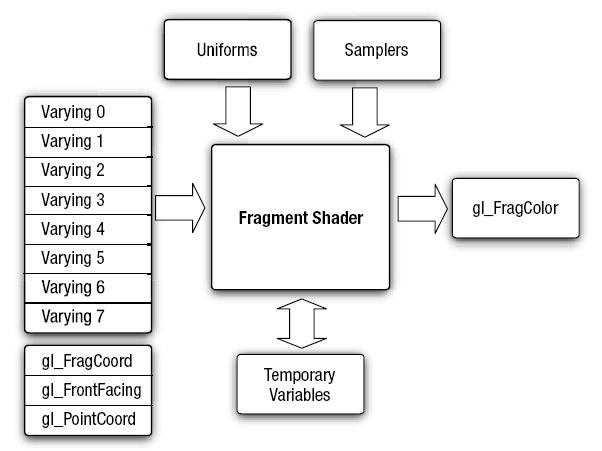
\includegraphics[width=11.5cm]{img/FragmentShader.jpg}
\caption{OpenGL ES 2.0 Fragmen Shaders}
\end{figure}

Algunas de las características que pueden ser implementadas en el fragment shader son la aplicación de mapeos usando texturas, simulación de efectos de niebla, etc.

\subsubsection{Per-Fragment}

En esta última fase se genera el buffer final, equivalente a los píxeles de la pantalla. Sobre cada uno de los fragmentos se ejecutan los siguientes test, aunque inicialmente están todos deshabilitados:
\begin{itemize}
\item \textbf{Scissor box testing:} elimina todos los píxeles fuera del área de visualización, el cual se determina con las propiedades de la cámara.
\item \textbf{Stencil buffer testing:} genera una máscara de la imagen a partir de una función \texttt{glStencilFunc}. La aplicación más conocida de este stencil buffer consiste en la generación de sombras.
\item \textbf{Depth buffer testing:} elimina todos aquellos fragmentos que no están visibles al ser ocultados por otros.
\item \textbf{Blending:} fusiona el color de los segmentos que se solapen en pantalla. A través de esta técnica se puede generar el efecto de transparencia de elementos como el cristal.
\item \textbf{Dithering:} ajusta los colores disponibles que no se adaptan a los colores que han sido calculados con él modelo de iluminación. Éste tipo de técnica consiste en intercalar los píxeles para que visualmente ofrezca un color similar al que deseamos.
\end{itemize}


\begin{figure}[H]
\centering
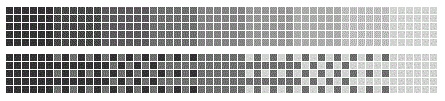
\includegraphics[width=11.5cm]{img/dithering.jpg}
\caption{Ejemplo de dithering sobre escala de grises}
\end{figure}
